
\begin{enumerate}
    \item As shown schematically in the figure, two vessels contain water solutions (at temperature \( T \)) of potassium permanganate (KMnO\(_4\)) of different concentrations \( n_1 \) and \( n_2 \) (\( n_1 > n_2 \)) molecules per unit volume with \( \Delta n = (n_1 - n_2) \ll n_1 \). When they are connected by a tube of small length \( l \) and cross-sectional area \( S \), KMnO\(_4\) starts to diffuse from the left to the right vessel through the tube. Consider the collection of molecules to behave as dilute ideal gases and the difference in their partial pressure in the two vessels causing the diffusion. The speed \( v \) of the molecules is limited by the viscous force \( -\beta v \) on each molecule, where \( \beta \) is a constant. Neglecting all terms of the order \( (\Delta n)^2 \), which of the following is/are correct? (\( k_B \) is the Boltzmann constant)
        \begin{tasks}(2)
            \task the force causing the molecules to move across the tube is \( \Delta nk_BTS \)
            \task force balance implies \( n_1\beta vl = \Delta nk_BT \)
            \task total number of molecules going across the tube per sec is \( \left(\frac{\Delta n}{l}\right) \left(\frac{k_BT}{\beta}\right) S \)
            \task rate of molecules getting transferred through the tube does not change with time
        \end{tasks}
\end{enumerate}

\begin{center}
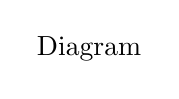
\begin{tikzpicture}
\node {Diagram};
\end{tikzpicture}
\end{center}
